\documentclass{beamer}
\usepackage{graphicx}
\usepackage{xcolor}
\usepackage{tikz}

% 自定义颜色
\definecolor{purpleblue}{RGB}{80, 80, 180}
\definecolor{lightgray}{RGB}{230, 230, 230}
\definecolor{novelPurple}{RGB}{98, 54, 255} 
\definecolor{darkgray}{RGB}{50, 50, 50}

% 主题设置
\usetheme{Madrid}  
\usecolortheme{dolphin} 

% 设置字体（移除 fontspec，确保 pdfLaTeX 兼容）
\setbeamerfont{title}{size=\Large,series=\bfseries}
\setbeamerfont{frametitle}{size=\LARGE,series=\bfseries}
\setbeamercolor{frametitle}{fg=white, bg=novelPurple}
\setbeamercolor{title}{fg=white, bg=purpleblue}

% 封面信息
\title[SAT Unit 4.1 Volume and Area]{\textbf{SAT Unit 4.1\\ Volume and Area}}
\author{\textbf{Jack Zeng}}
\institute{\textcolor{white}{\textbf{Novel Prep}}}
\date{\today} 

\begin{document}

% --- Title Slide ---
\begin{frame}
    \titlepage
    \vfill
    \begin{flushright}
        \textcolor{purpleblue}{\Huge \textbf{Novel Prep}}
    \end{flushright}
\end{frame}


\begin{frame}
    \begin{tikzpicture}[remember picture, overlay]
        % 设置浅色渐变背景
        \shade[top color=softPurple, bottom color=softGray] 
            (current page.north west) rectangle (current page.south east);
        
        % 添加高斯模糊光晕
        \fill[white, opacity=0.3] (current page.center) circle (4cm);
        
        % 主标题
        \node[align=center] at (current page.center) {
            {\Huge\bfseries\textcolor{purpleblue}{Novel Prep}} \\[0.5cm]
            {\Large\itshape\textcolor{lightText}{Excellence in SAT Prep}}
        };

        % 添加柔和光点（点缀）
        \foreach \x in {1,2,3,4,5} {
            \fill[purpleblue, opacity=0.2] (rand*10-5, rand*7-3.5) circle (0.1+\x*0.05);
        }

        ;
    \end{tikzpicture}
\end{frame}

\begin{frame}{Overview}
    \tableofcontents
\end{frame}


\begin{frame}
\section{Perimeter and Area}
    \begin{tikzpicture}[remember picture, overlay]
        \shade[top color=softPurple, bottom color=softGray] 
            (current page.north west) rectangle (current page.south east);
        \fill[white, opacity=0.3] (current page.center) circle (4cm);
        
        \node[align=center] at (current page.center) {
            {\Huge\bfseries\textcolor{purpleblue}{Perimeter and Area}} \\[0.5cm]
            {\Large\itshape\textcolor{lightText}{Excellence in SAT Prep}}
        };
        \foreach \x in {1,2,3,4,5} {
            \fill[purpleblue, opacity=0.2] (rand*10-5, rand*7-3.5) circle (0.1+\x*0.05);
        }
        ;
    \end{tikzpicture}
\end{frame}





% --- Slide: Perimeter Formulas ---
\begin{frame}{\textbf{Perimeter Formulas}}
    \begin{itemize}
        \item Square: \( P = 4s \)
        \item Rectangle: \( P = 2(l + w) \)
        \item Triangle: \( P = a + b + c \)
        \item Circle (Circumference): \( P = 2\pi r \) or \( P = \pi d \)
    \end{itemize}
    \vspace{0.5cm}
    \centering
    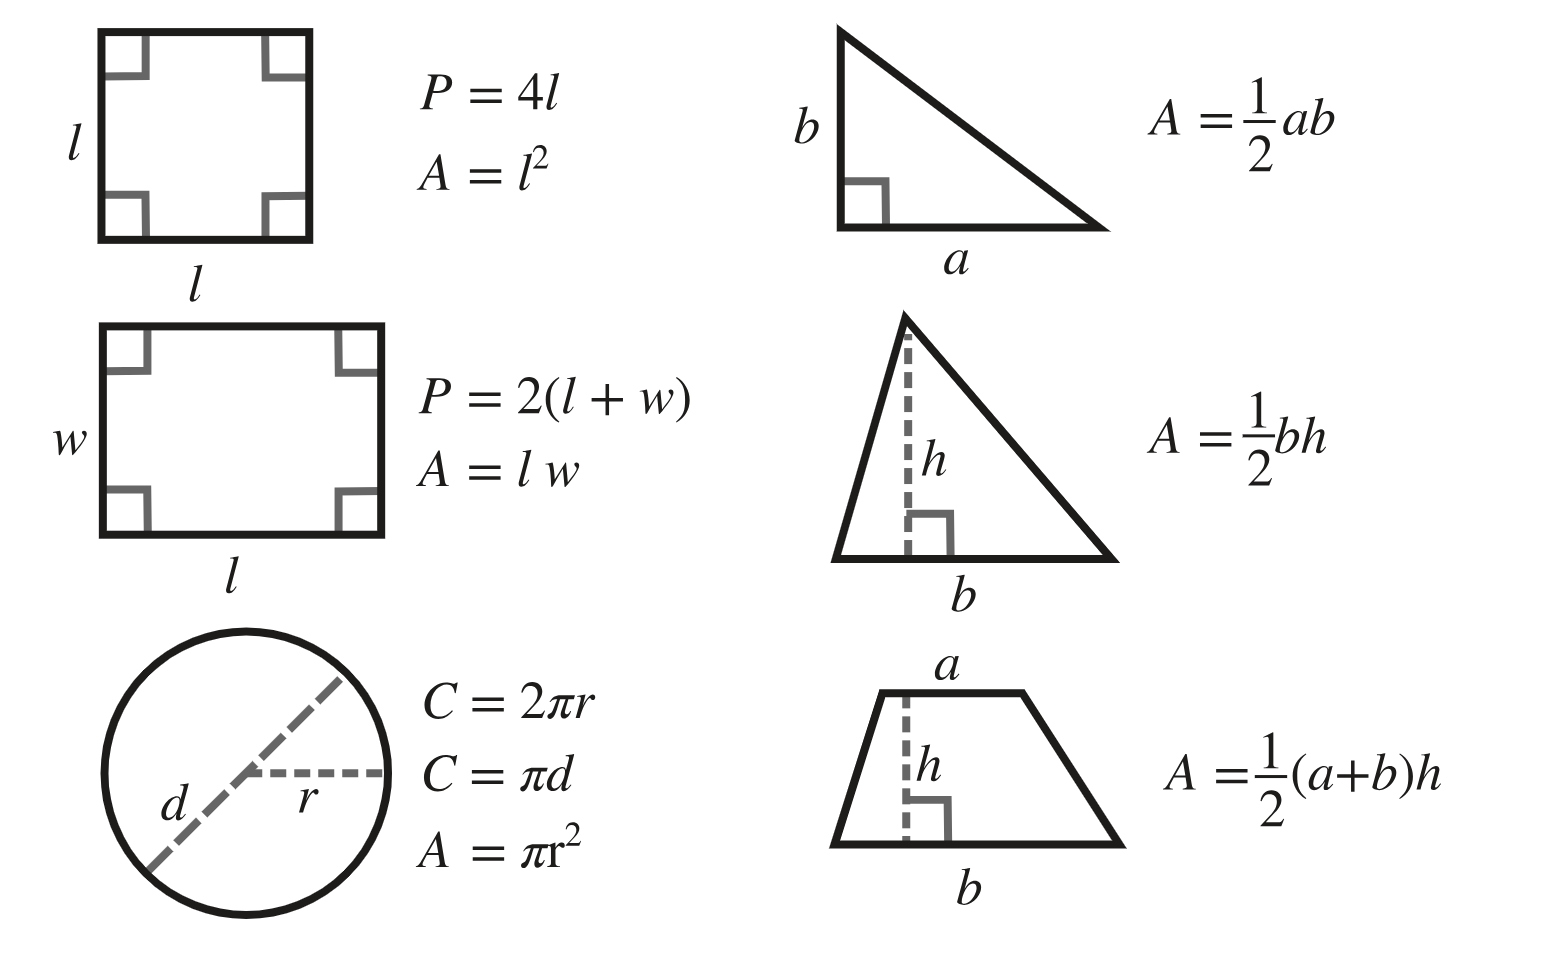
\includegraphics[width=0.6\linewidth]{E4.png} % Replace with correct figure
\end{frame}

% --- Slide: Area Formulas ---
\begin{frame}{\textbf{Area Formulas}}
    \begin{itemize}
        \item Square: \( A = s^2 \)
        \item Rectangle: \( A = lw \)
        \item Triangle: \( A = \frac{1}{2} bh \)
        \item Parallelogram: \( A = bh \)
        \item Trapezoid: \( A = \frac{1}{2} (b_1 + b_2) h \)
        \item Circle: \( A = \pi r^2 \)
    \end{itemize}
    \vspace{0.5cm}
    \centering
    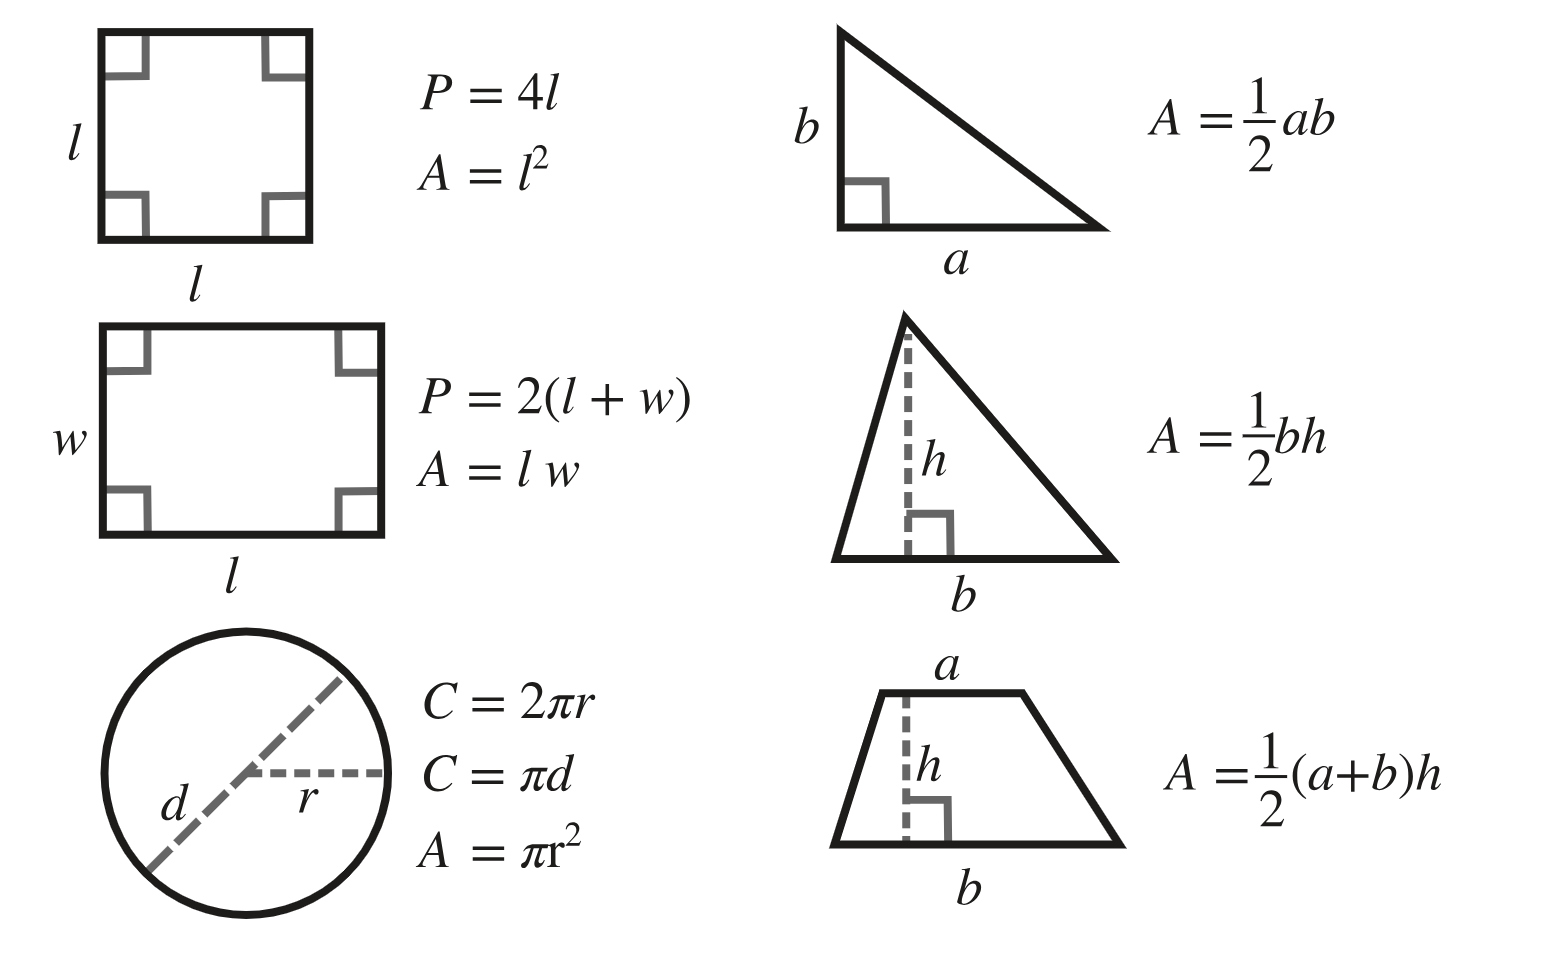
\includegraphics[width=0.6\linewidth]{E4.png} % Replace with correct figure
\end{frame}


\begin{frame}
\section{Volume}
    \begin{tikzpicture}[remember picture, overlay]
        \shade[top color=softPurple, bottom color=softGray] 
            (current page.north west) rectangle (current page.south east);
        \fill[white, opacity=0.3] (current page.center) circle (4cm);
        
        \node[align=center] at (current page.center) {
            {\Huge\bfseries\textcolor{purpleblue}{Volume}} \\[0.5cm]
            {\Large\itshape\textcolor{lightText}{Excellence in SAT Prep}}
        };
        \foreach \x in {1,2,3,4,5} {
            \fill[purpleblue, opacity=0.2] (rand*10-5, rand*7-3.5) circle (0.1+\x*0.05);
        }
        ;
    \end{tikzpicture}
\end{frame}

% --- Slide: Volume Formulas ---
\begin{frame}{\textbf{Prism Volume}}
    \textbf{Definition:} A prism is a three-dimensional shape with two parallel and congruent bases.  
    The volume of a prism is calculated using the formula:
    
    \[
    V_{\text{PRISM}} = Bh
    \]
    
    where:
    \begin{itemize}
        \item \( B \) is the **Area of the Base**.
        \item \( h \) is the **Height of the Prism** (one of its lateral sides).
    \end{itemize}
    
   \begin{center}
       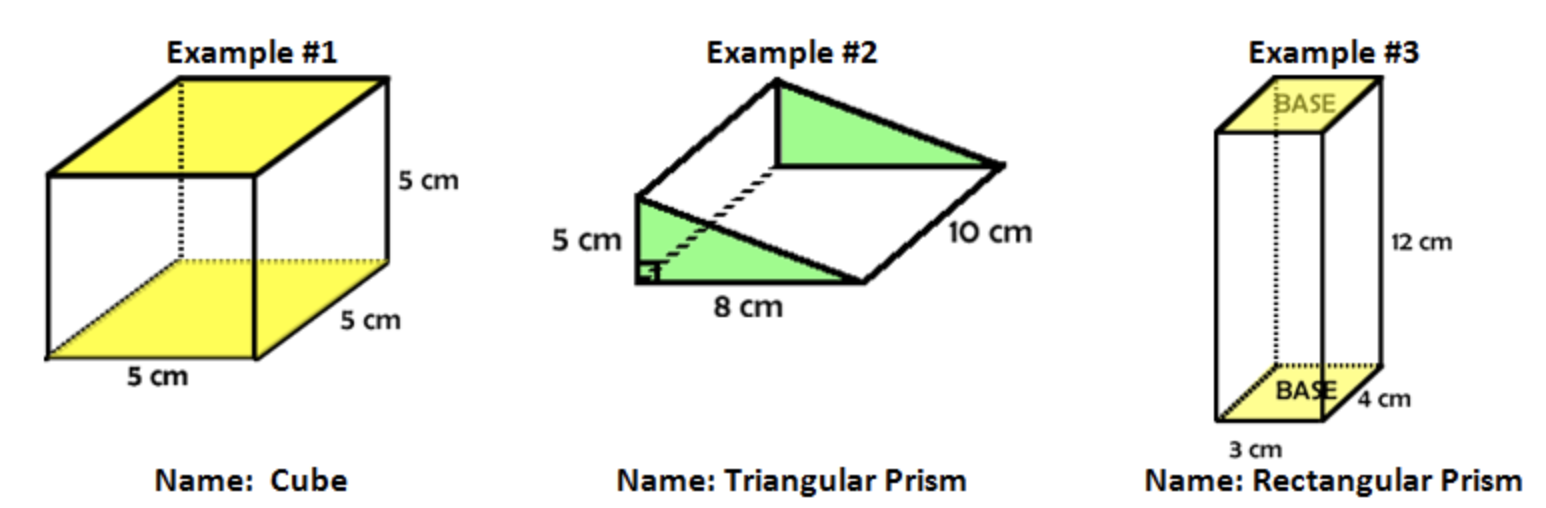
\includegraphics[width=0.95\linewidth]{E5.png}
   \end{center}
\end{frame}

\begin{frame}{Surface Area of a Cube}
\textbf{Question:}  
A cube has a volume of 42,875 cubic inches. What is the surface area, in square inches, of the cube?
\end{frame}

\begin{frame}{Solution}
\textbf{Solution:}
\begin{itemize}
    \item Let \( s \) be the side length of the cube.
    \item Given:
    \[
    s^3 = 42,875
    \]
    \item Solve for \( s \):
    \[
    s = \sqrt[3]{42,875} \approx 35 \text{ inches}
    \]
    \item Surface area of the cube:
    \[
    \text{Surface Area} = 6s^2 = 6 \times (35)^2 = 6 \times 1225 = 7350 \text{ in}^2
    \]
\end{itemize}

\textbf{Answer:} \( 7350 \) square inches.
\end{frame}







\begin{frame}{\textbf{Cylinder Volume Calculation}}
    \textbf{Definition:} A cylinder is a three-dimensional shape with two parallel, congruent circular bases.  
    The volume of a cylinder is calculated using the formula:

    \[
    V_{\text{CYLINDER}} = Bh
    \]
    \[
    V_{\text{CYLINDER}} = \pi r^2 h
    \]

    where:
    \begin{itemize}
        \item \( B \) is the **Area of the Base** (which is a circle, so \( B = \pi r^2 \)).
        \item \( h \) is the **Height of the Cylinder**, the perpendicular distance between the two circular bases.
    \end{itemize}

      \begin{center}
          
    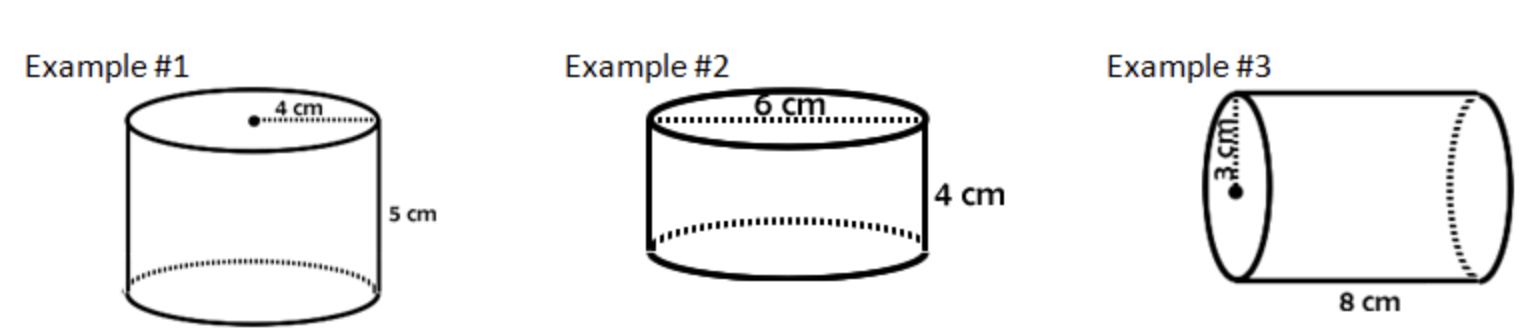
\includegraphics[width=0.9\linewidth]{E6.png} % Replace with correct figure
    \end{center}
\end{frame}
\begin{frame}{Cylinder Problem}
\textbf{Question:}  
A cylinder has a volume of \(980\pi\) cubic feet and a height of 5 feet. What is the base diameter, in feet, of the cylinder?
\end{frame}

\begin{frame}{Solution}
\textbf{Solution:}
\begin{itemize}
    \item Volume of a cylinder:
    \[
    V = \pi r^2 h
    \]
    \item Given:
    \[
    980\pi = \pi r^2 \times 5
    \]
    \item Simplify:
    \[
    r^2 = \frac{980}{5}
    \]
    \[
    r^2 = 196
    \]
    \[
    r = 14 \text{ feet}
    \]
    \item Diameter:
    \[
    d = 2r = 2 \times 14 = 28 \text{ feet}
    \]
\end{itemize}

\textbf{Answer:} \(28\) feet
\end{frame}




\begin{frame}{\textbf{Pyramid Volume Calculation}}
    \textbf{Definition:} A pyramid is a three-dimensional shape with a polygonal base and triangular faces that converge at a single point (the apex).  
    The volume of a pyramid is given by the formula:

    \[
    V_{\text{PYRAMID}} = \frac{1}{3} Bh
    \]

    where:
    \begin{itemize}
        \item \( B \) is the \textbf{Area of the Base}.
        \item \( h \) is the Height of the Pyramid, the perpendicular distance from the base to the apex.
        \item The volume of a pyramid is always \textbf{one-third} of the volume of a prism with the same base and height.
    \end{itemize}
    
    \begin{center}
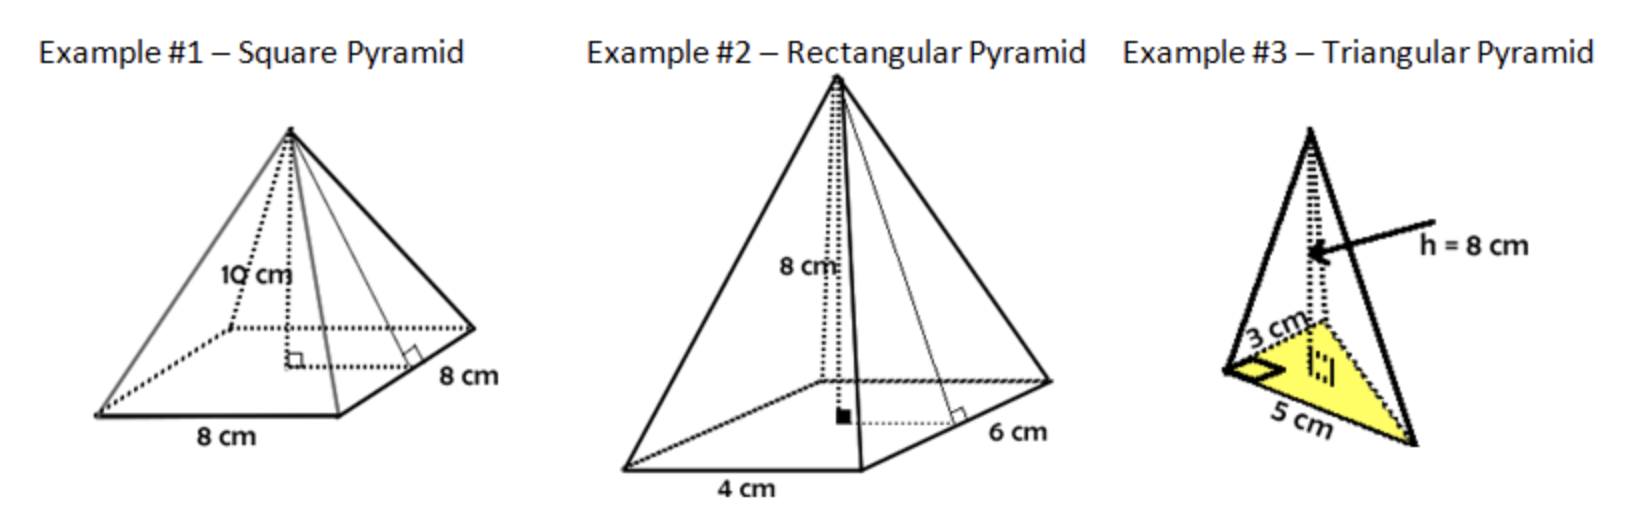
\includegraphics[width=0.6\linewidth]{E7.png} 

    \end{center}
\end{frame}


\begin{frame}{Volume of a Pyramid}
\textbf{Question:}  
A right square pyramid has a height of 33 centimeters (cm) and a square base with a side length of 14 cm. What is the volume, in cm³, of this pyramid?
\end{frame}


\begin{frame}{Solution}
\textbf{Solution:}
\begin{itemize}
    \item The formula for the volume of a right square pyramid is:
    \[
    V = \frac{1}{3} \times \text{Base Area} \times \text{Height}
    \]
    \item Base area:
    \[
    \text{Base Area} = 14 \times 14 = 196 \text{ cm}^2
    \]
    \item Therefore:
    \[
    V = \frac{1}{3} \times 196 \times 33
    \]
    \[
    V = \frac{1}{3} \times 6468
    \]
    \[
    V = 2156 \text{ cm}^3
    \]
\end{itemize}

\textbf{Answer:} \( 2156 \text{ cm}^3 \)
\end{frame}

\begin{frame}{Right Triangular Pyramid}

\textbf{What is a Right Triangular Pyramid?}
\begin{itemize}
    \item A three-dimensional solid with a triangular base.
    \item The apex (top point) is directly above the centroid of the triangular base.
    \item Has 4 faces: 1 triangular base and 3 triangular lateral faces.
    \item All lateral edges meet at the apex.
\end{itemize}


\begin{center}

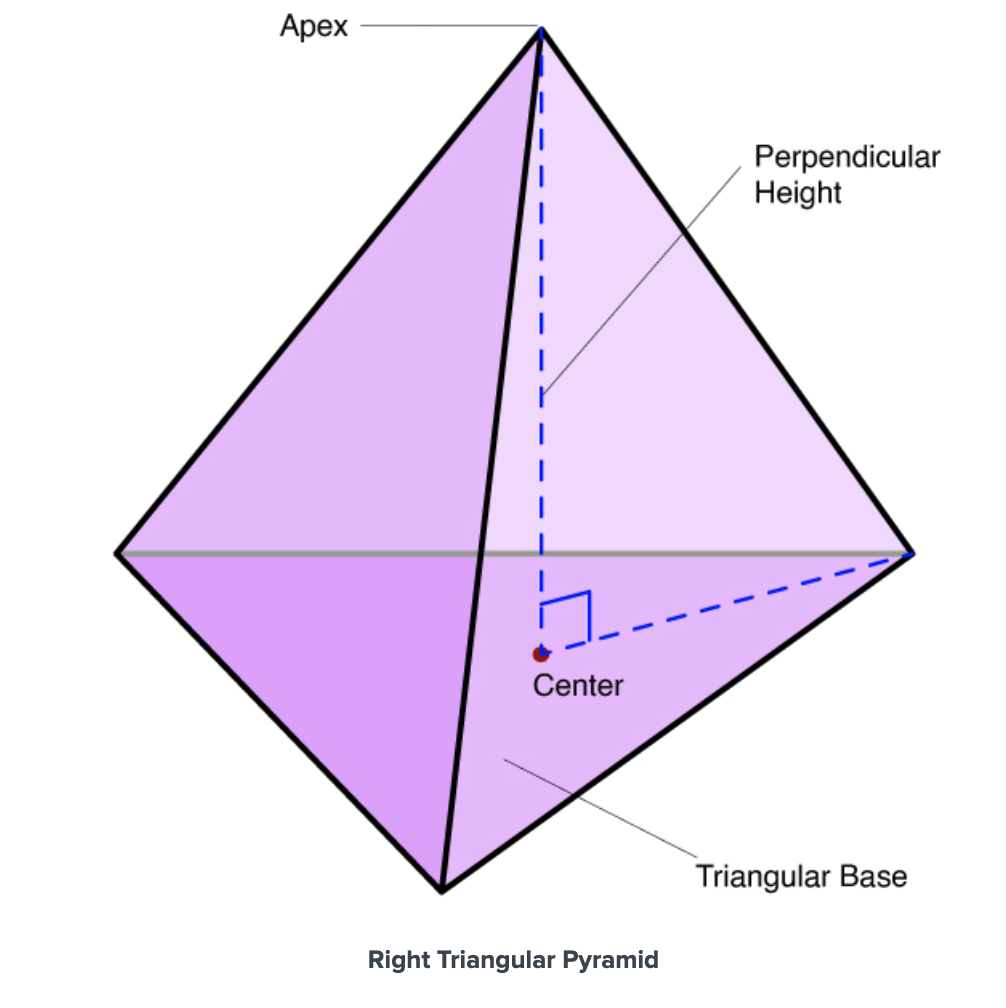
\includegraphics[width=0.40\linewidth]{E82.png}
\end{center}



\end{frame}

\begin{frame}{Right Triangular Pyramid}
\small

\textbf{Volume Formula:}
\[
V = \frac{1}{3} \times \text{Base Area} \times \text{Height}
\]
Where:
\begin{itemize}

    \item Height = perpendicular distance from the apex to the base
\end{itemize}

\vspace{1em}
\textbf{Surface Area Formula:}
\[
\text{Surface Area} = \text{Base Area} + \text{Sum of lateral face areas}
\]
Each lateral face is a triangle: $\frac{1}{2} \times \text{base} \times \text{slant height}$


\begin{center}

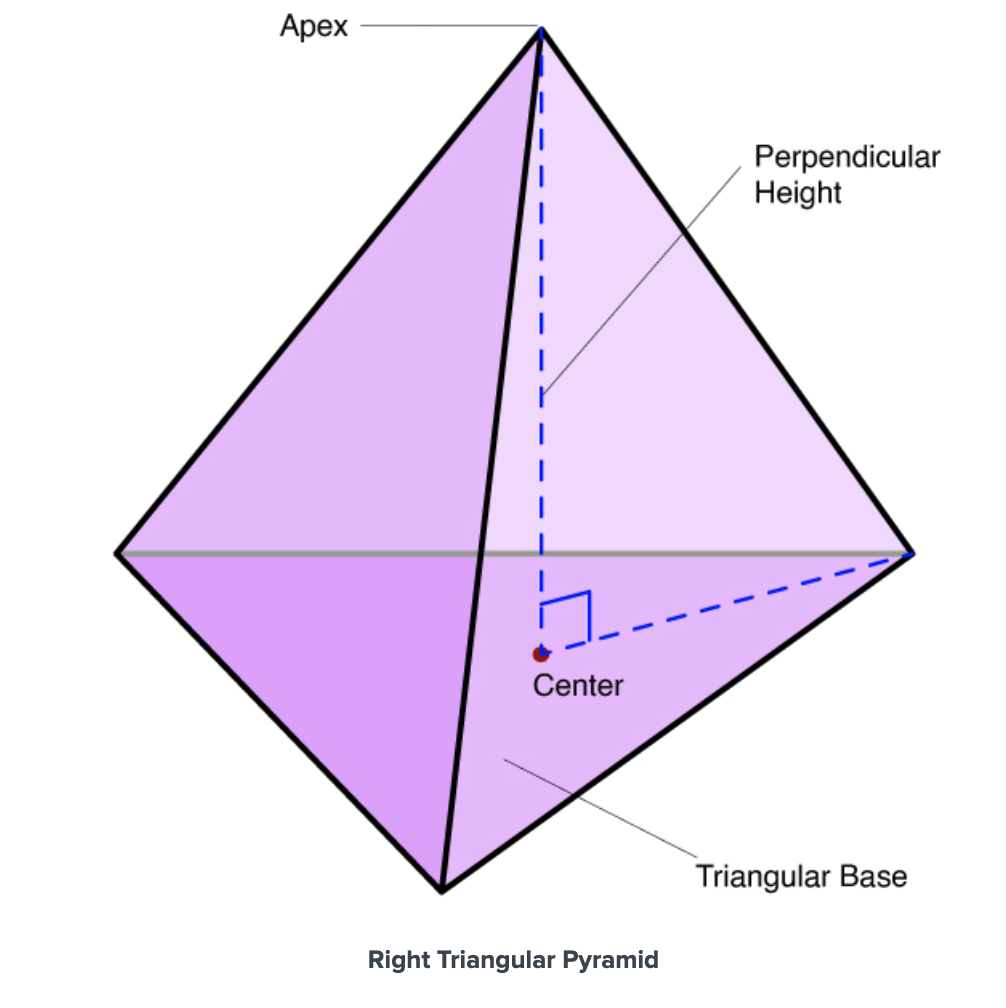
\includegraphics[width=0.3\linewidth]{E82.png}
\end{center}

\end{frame}




\begin{frame}
\section{Density}
    \begin{tikzpicture}[remember picture, overlay]
        \shade[top color=softPurple, bottom color=softGray] 
            (current page.north west) rectangle (current page.south east);
        \fill[white, opacity=0.3] (current page.center) circle (4cm);
        
        \node[align=center] at (current page.center) {
            {\Huge\bfseries\textcolor{purpleblue}{Density}} \\[0.5cm]
            {\Large\itshape\textcolor{lightText}{Excellence in SAT Prep}}
        };
        \foreach \x in {1,2,3,4,5} {
            \fill[purpleblue, opacity=0.2] (rand*10-5, rand*7-3.5) circle (0.1+\x*0.05);
        }
        ;
    \end{tikzpicture}
\end{frame}




\begin{frame}{Density}
\textbf{Definition:} Density is a measure of how much mass is contained in a given volume.

\begin{block}{Formula}
\[
\text{Density} = \frac{\text{Mass}}{\text{Volume}}
\]
where:
\begin{itemize}
    \item Mass is typically measured in grams (g) or kilograms (kg).
    \item Volume is typically measured in cubic centimeters (cm³) or cubic meters (m³).
\end{itemize}
\end{block}

\pause
\textbf{Example:}
\begin{itemize}
    \item A rock has a mass of 200 grams and a volume of 50 cm³.
    \item Calculate the density:
    \[
    \text{Density} = \frac{200 \text{ g}}{50 \text{ cm}^3} = 4 \text{ g/cm}^3
    \]
\end{itemize}


\end{frame}





\begin{frame}{Density Problem}
\textbf{Question:}  
The mass of a foam block is 8 kilograms. The volume of the block is 20 cubic meters. What is the density, in kilograms per cubic meter, of the block?

\begin{enumerate}[A.]
    \item 0.4
    \item 2.5
    \item 12
    \item 28
\end{enumerate}
\end{frame}

\begin{frame}{Solution}
\textbf{Solution:}  
Density is given by:
\[
\text{Density} = \frac{\text{Mass}}{\text{Volume}} = \frac{8 \text{ kg}}{20 \text{ m}^3} = 0.4 \text{ kg/m}^3.
\]

\textbf{Answer:} A.
\end{frame}




\begin{frame}
\section{Ratio of Length, Area, and Volume}
    \begin{tikzpicture}[remember picture, overlay]
        \shade[top color=softPurple, bottom color=softGray] 
            (current page.north west) rectangle (current page.south east);
        \fill[white, opacity=0.3] (current page.center) circle (4cm);
        
        \node[align=center] at (current page.center) {
            {\LARGE\bfseries\textcolor{purpleblue}{Ratio of Length, Area, and Volume}} \\[0.5cm]
            {\Large\itshape\textcolor{lightText}{Excellence in SAT Prep}}
        };
        \foreach \x in {1,2,3,4,5} {
            \fill[purpleblue, opacity=0.2] (rand*10-5, rand*7-3.5) circle (0.1+\x*0.05);
        }
        ;
    \end{tikzpicture}
\end{frame}


\begin{frame}{\textbf{Ratio of Length, Area, and Volume}}

    \textbf{Concept:}  
    When a geometric shape is scaled by a factor of \( k \), the following relationships hold:

    \vspace{0.3cm}
    \begin{itemize}
        \item \textbf{Length Ratio:} If the scale factor is \( k \), then all linear measurements (length, width, height, radius, etc.) change by a factor of \( k \).
        \[
        \text{New Length} = k \times \text{Original Length}
        \]
        
        \item \textbf{Area Ratio:} The area of a shape is proportional to the square of the scale factor.
        \[
        \text{New Area} = k^2 \times \text{Original Area}
        \]

        \item \textbf{Volume Ratio:} The volume of a three-dimensional shape is proportional to the cube of the scale factor.
        \[
        \text{New Volume} = k^3 \times \text{Original Volume}
        \]
    \end{itemize}
\end{frame}

% --- Question Frame ---
\begin{frame}{\textbf{Question: Ratio of Length, Area, and Volume}}
    Suppose a cube has an original edge length of \( 2 \) cm, and we scale it up by a factor of \( k = 3 \).  
    How do the length, area, and volume change under this transformation?

    \vspace{0.5cm}
    \textbf{Options:}
    \begin{enumerate}
        \item[A] Length scales by \( k \), area scales by \( k^2 \), volume scales by \( k^3 \).
        \item[B] Length scales by \( k^2 \), area scales by \( k^3 \), volume scales by \( k^4 \).
        \item[C] Length scales by \( k \), area scales by \( k^3 \), volume scales by \( k^2 \).
        \item[D] Length scales by \( k^3 \), area scales by \( k^2 \), volume scales by \( k \).
    \end{enumerate}
\end{frame}

% --- Answer Explanation ---
\begin{frame}{\textbf{Answer Explanation: Ratio of Length, Area, and Volume}}
    \textbf{Correct Answer: \textcolor{novelPurple}{\(\mathbf{k, k^2, k^3}\)}}  

    \vspace{0.3cm}
    \textbf{Solution:}  
    When a shape is scaled by a factor of \( k \):

    \begin{itemize}
        \item \textbf{Length:} Scales by \( k \).
        \[
        \text{New Length} = k \times \text{Original Length}
        \]

        \item \textbf{Area:} Scales by \( k^2 \).
        \[
        \text{New Area} = k^2 \times \text{Original Area}
        \]

        \item \textbf{Volume:} Scales by \( k^3 \).
        \[
        \text{New Volume} = k^3 \times \text{Original Volume}
        \]
    \end{itemize}



    \textbf{Final Answer:} \( \boxed{k, k^2, k^3} \).
\end{frame}



% --- Question Frame ---
\begin{frame}{\textbf{Question: Finding the Volume of a Cube}}
    A cube has a surface area of \( 54 \) square meters.  
    What is the volume, in cubic meters, of the cube?

    \vspace{0.5cm}
    \textbf{Options:}
    \begin{enumerate}
        \item[A.] 18
        \item[B.] 27
        \item[C.] 36
        \item[D.] 81
    \end{enumerate}
\end{frame}

% --- Answer Explanation ---
\begin{frame}{\textbf{Answer Explanation: Finding the Volume of a Cube}}
    \textbf{Correct Answer: \textcolor{novelPurple}{\( \mathbf{B} \)}}  

    \vspace{0.3cm}
    \textbf{Solution:}  
    A cube has 6 identical square faces. If the total surface area is given as:

    \[
    6s^2 = 54
    \]

    Solve for \( s \):

    \[
    s^2 = \frac{54}{6} = 9
    \]

    \[
    s = \sqrt{9} = 3
    \]

    \vspace{0.3cm}
    Now, calculate the volume:

    \[
    V = s^3 = 3^3 = 27
    \]

    \textbf{Final Answer:} \( \boxed{27} \).
\end{frame}














% --- Question Frame ---
\begin{frame}{\textbf{Question: Area of a Scaled Poster}}
    A rectangular poster has an area of **360** square inches.  
    A copy of the poster is made in which the **length** and **width**  
    of the original poster are each increased by **20\%**.  

    \vspace{0.5cm}
    What is the area of the copy, in square inches?
\end{frame}

% --- Answer Explanation ---
\begin{frame}{\textbf{Answer Explanation: Area of a Scaled Poster}}
    \textbf{Solution:}  

    \vspace{0.3cm}
    \textbf{Step 1: Define Scaling Factor}  
    Since both length and width increase by \( 20\% \),  
    the new dimensions are scaled by:

    \[
    k = 1.2
    \]

    \vspace{0.3cm}
    \textbf{Step 2: Apply Area Scaling Formula}  
    Since **area scales by \( k^2 \)**:

    \[
    \text{New Area} = 360 \times (1.2)^2
    \]

    \[
    = 360 \times 1.44 = 518.4
    \]

    \vspace{0.3cm}
    \textbf{Final Answer:} \( \boxed{518.4} \) square inches.
\end{frame}


% --- Summary Slide ---
\begin{frame}{\textbf{Key Takeaways}}
    \begin{itemize}
        \item Memorizing perimeter, area, and volume formulas is crucial.
        \item Understanding the ratio between the length, Area, and the Volume.
        \item Recognizing shapes and their properties in SAT problems.
    \end{itemize}
    \vfill
    \centering
    \textcolor{novelPurple}{\Huge \textbf{Practice Makes Perfect!}}
\end{frame}

\begin{frame}
\section{Practices}
    \begin{tikzpicture}[remember picture, overlay]
     
        \shade[top color=softPurple, bottom color=softGray] 
            (current page.north west) rectangle (current page.south east);
        
       
        \fill[white, opacity=0.3] (current page.center) circle (4cm);
        

        \node[align=center] at (current page.center) {
            {\Huge\bfseries\textcolor{purpleblue}{Practices}} \\[0.5cm]
            {\Large\itshape\textcolor{lightText}{Excellence in SAT Prep}}
        };


        \foreach \x in {1,2,3,4,5} {
            \fill[purpleblue, opacity=0.2] (rand*10-5, rand*7-3.5) circle (0.1+\x*0.05);
        }

        ;
    \end{tikzpicture}
\end{frame}


\begin{frame}{Cube Problem}
\textbf{Question:}  
The surface area, in square inches, of a cube can be represented by the expression \(24a^2\), where \(a\) is a positive constant. Which expression represents the volume, in cubic inches, of the cube?

\begin{itemize}
    \item[A)] \(8a^3\)
    \item[B)] \(16a^3\)
    \item[C)] \(64a^6\)
    \item[D)] \(216a^6\)
\end{itemize}
\end{frame}


\begin{frame}{Solution}
\textbf{Solution:}
\begin{itemize}
    \item Let \(s\) be the side length of the cube.
    \item The surface area of the cube is \(6s^2 = 24a^2\).
    \item Solve for \(s^2\):
    \[
    s^2 = \frac{24a^2}{6} = 4a^2
    \]
    \item Then:
    \[
    s = 2a
    \]
    \item The volume of the cube:
    \[
    V = s^3 = (2a)^3 = 8a^3
    \]
\end{itemize}

\textbf{Answer:} \(8a^3\) (Choice A)
\end{frame}



\begin{frame}{Volume of a Cylinder}
\textbf{Question:}  
Given the function \( f(x) = \pi x^3 + \pi x^2 \), where \( f \) represents the volume (in cubic feet) of a right circular cylinder with radius \( x \) feet, which expression represents the height (in feet) of the cylinder?

\begin{itemize}
    \item[A)] \( x + 1 \)
    \item[B)] \( \pi x^3 \)
    \item[C)] \( x \)
    \item[D)] \( x^3 + 1 \)
\end{itemize}
\end{frame}


\begin{frame}{Solution}
\textbf{Solution:}
\begin{itemize}
    \item The volume of a right circular cylinder is given by:
    \[
    V = \pi r^2 h
    \]
    \item Comparing with \( f(x) = \pi x^3 + \pi x^2 \), notice that:
    \[
    f(x) = \pi x^2 (x + 1)
    \]
    \item Therefore, \( r = x \) and \( h = x + 1 \).
\end{itemize}

\textbf{Answer:} \( x + 1 \) (Choice A)
\end{frame}


\begin{frame}{Rectangle Perimeter Problem}
\textbf{Question:}
Identical rectangles \(X\) and \(Y\) each have an area of \(\frac{49}{5}\) square meters and a perimeter of \(P\) meters. If one of the shorter sides of rectangle \(X\) is glued to one of the shorter sides of rectangle \(Y\), the resulting rectangle has a perimeter of \(\frac{14}{9}P\) meters. What is the value of \(P\)?
\end{frame}



\begin{frame}{Solution}
\footnotesize
\textbf{Solution:}
\begin{itemize}
    \item Let \(l\) and \(w\) be the length and width of each rectangle.
    \item Then:
    \[
    lw = \frac{49}{5} \quad \text{and} \quad 2(l+w) = P
    \]
    \item When glued along the shorter side:
    \[
    \text{New perimeter} = 2(l + 2w)
    \]
    \item Given:
    \[
    2(l + 2w) = \frac{14}{9}P
    \]
    \item But \(P = 2(l+w)\) so:
    \[
    2(l + 2w) = \frac{14}{9} \cdot 2(l+w)
    \]
    \item Dividing both sides by 2:
    \[
    l + 2w = \frac{14}{9}(l+w)
    \]
    \item Solve:
    \[
    9(l + 2w) = 14(l + w)
    \]
    \[
    9l + 18w = 14l + 14w
    \]
    \[
    4w = 5l
    \]
  \end{itemize}
\end{frame}

\begin{frame}{Solution}

\footnotesize

\begin{itemize}
      \item From \(lw = \frac{49}{5}\):
    \[
    l \left(\frac{5l}{4}\right) = \frac{49}{5}
    \]
    \[
    \frac{5l^2}{4} = \frac{49}{5}
    \]
    \[
    l^2 = \frac{49}{5} \cdot \frac{4}{5} = \frac{196}{25}
    \]
    \[
    l = \frac{14}{5}
    \]
    \item Then:
    \[
    w = \frac{5l}{4} = \frac{5 \cdot \frac{14}{5}}{4} = \frac{14}{4} = 3.5
    \]
    \item Hence:
    \[
    P = 2(l + w) = 2\left(\frac{14}{5} + 3.5\right) = 2\left(\frac{14}{5} + \frac{7}{2}\right)
    \]
    \[
    = 2\left(\frac{28}{10} + \frac{35}{10}\right) = 2\left(\frac{63}{10}\right) = \frac{126}{10} = 12.6
    \]
    
\textbf{Answer:} \( P = 12.6 \) meters.
\end{itemize}


\end{frame}










\begin{frame}{}
    \begin{tikzpicture}[remember picture, overlay]
        % 背景渐变色：蓝紫到白
        \shade[top color=novelPurple!40, bottom color=white]
            (current page.north west) rectangle (current page.south east);

        % 中心柔光
        \fill[white, opacity=0.15] (current page.center) circle (5cm);

        % 柔和光点点缀
        \foreach \x in {1,2,3,4,5} {
            \fill[novelPurple, opacity=0.12] (rand*10-5, rand*7-3.5) circle (0.1+\x*0.05);
        }
    \end{tikzpicture}

    \centering
    \vspace{5em}

    {\Huge \textbf{\textcolor{novelPurple}{Thank You!}}} \\[1em]
    {\large \textcolor{gray}{We appreciate your time and focus.}} \\[3em]

    {\LARGE \textbf{\textcolor{novelPurple}{\textsf{Novel Prep}}}}

    \vfill
\end{frame}



\end{document}